\documentclass[a4paper,12pt]{article}
\usepackage[a4paper,top=1.3cm,bottom=2cm,left=1.5cm,right=1.5cm,marginparwidth=0.75cm]{geometry}
\usepackage{cmap}
\usepackage{mathtext}
\usepackage[T2A]{fontenc}
\usepackage[utf8]{inputenc}
\usepackage[english,russian]{babel}
\usepackage{siunitx}
\usepackage{enumitem}
\usepackage{placeins}

\usepackage{graphicx}

\usepackage{wrapfig}
\usepackage{tabularx}
\usepackage{multirow}

\usepackage{hyperref}
\usepackage[rgb]{xcolor}
\hypersetup{
colorlinks=true,urlcolor=blue
}
\usepackage{siunitx}
\usepackage{geometry}
\usepackage{amsmath,amsfonts,amssymb,physics,amsthm,mathtools}
\usepackage{icomma}
\mathtoolsset{showonlyrefs=false}
\usepackage{euscript}
\usepackage{mathrsfs}
\DeclareMathOperator{\sgn}{\mathop{sgn}}
\newcommand*{\hm}[1]{#1\nobreak\discretionary{}
{\hbox{$\mathsurround=0pt #1$}}{}}

%%% Заголовок
\author{Макаров Лев Евгеньевич}
\title{Вопрос по выбору\\
Метаматериалы}

\date{\today}

\begin{document}


\begin{titlepage}
	\begin{center}
		{\large МОСКОВСКИЙ ФИЗИКО-ТЕХНИЧЕСКИЙ ИНСТИТУТ (НАЦИОНАЛЬНЫЙ ИССЛЕДОВАТЕЛЬСКИЙ УНИВЕРСИТЕТ)}
	\end{center}
	\begin{center}
		{\large Физтех-школа фотоники, электроники и молекулярной физики}
	\end{center}
	
	
	\vspace{4.5cm}
	{\huge
		\begin{center}
			{\bf Вопрос по выбору}\\
			Метаматериалы
		\end{center}
	}
	\vspace{2cm}
	\begin{flushright}
		{\LARGE Автор:\\ Макаров Лев Евгеньевич \\
			\vspace{0.2cm}
			Б04-306}
	\end{flushright}
	\vspace{8cm}
	\begin{center}
		Долгопрудный 2025
	\end{center}
\end{titlepage}

\section{Введение}
Метаматериалы — это искусственные среды, обладающие уникальными электромагнитными свойствами, включая возможность иметь одновременно отрицательные диэлектрическую ($\varepsilon$) и магнитную ($\mu$) проницаемости. Эти свойства приводят к феноменам, не встречающимся в природной оптике: отрицательный показатель преломления, обратный эффект Доплера, фокусировка плоской линзой и другие. В данном докладе будет подробно выведено волновое уравнение из уравнений Максвелла, рассмотрены фазовая и групповая скорости, импеданс среды, условия отражения и поглощения, а также особенности переноса энергии в левосторонних средах.

\section{Теоретическое введение}
Рассмотрим однородную, изотропную среду без свободных зарядов и токов. Уравнения Максвелла:
\begin{align}
    \nabla \cdot \vb{D} &= 0, & \nabla \cdot \vb{B} &= 0, \\
    \nabla \times \vb{E} &= -\pdv{\vb{B}}{t}, & \nabla \times \vb{H} &= \pdv{\vb{D}}{t}.
\end{align}
Поскольку $\vb{D} = \varepsilon \vb{E}$ и $\vb{B} = \mu \vb{H}$, можно записать:
\begin{equation}
    \nabla \times \vb{E} = -\mu \pdv{\vb{H}}{t}, \qquad
    \nabla \times \vb{H} = \varepsilon \pdv{\vb{E}}{t}.
\end{equation}
Взяв ротор от первого уравнения и подставив второе:
\begin{align*}
    \nabla \times (\nabla \times \vb{E}) &= -\mu \pdv{}{t}(\nabla \times \vb{H}) \\
    &= -\mu \varepsilon \pdv[2]{\vb{E}}{t}.
\end{align*}
Используя векторное тождество $\nabla \times (\nabla \times \vb{E}) = \nabla(\nabla \cdot \vb{E}) - \Delta \vb{E}$ и $\nabla \cdot \vb{E} = 0$, получаем:
\begin{equation}
    \Delta \vb{E} - \varepsilon\mu \pdv[2]{\vb{E}}{t} = 0.
\end{equation}
Аналогично выводится волновое уравнение для $\vb{H}$.


Пусть $\vb{E}(\vb{r},t) = \vb{E}_0(\vb{r})e^{-i\omega t}$. Подставляя в волновое уравнение:
\begin{equation}
    \Delta \vb{E}_0 + k^2 \vb{E}_0 = 0, \qquad k = \omega \sqrt{\varepsilon\mu}.
\end{equation}
Это уравнение Гельмгольца. Показатель преломления: $n = \pm\sqrt{\varepsilon \mu}$.

\subsection{Фазовая и групповая скорости}
Фазовая скорость:
\begin{equation}
    v_{\text{ф}} = \frac{\omega}{k} = \frac{c}{n},
\end{equation}
где $c = 1/\sqrt{\varepsilon_0 \mu_0}$. Групповая скорость:
\begin{equation}
    u = \pdv{\omega}{k} = \left(\pdv{k}{\omega}\right)^{-1} = \frac{c}{n + \omega \pdv{n}{\omega}}.
\end{equation}
В средах с $n<0$ фазовая и групповая скорости направлены противоположно.

\subsection{Импеданс и условия отражения}
Импеданс — это отношение амплитуд электрического и магнитного полей в плоской волне:
\begin{equation}
    Z = \frac{E}{H} = \sqrt{\frac{\mu}{\varepsilon}}.
\end{equation}
В волновой задаче на границе двух сред с импедансами $Z_1$ и $Z_2$ и нормальным падением волны, коэффициенты отражения и пропускания по амплитуде (для $E$-волны) находятся из условий непрерывности $E$ и $H$:
\begin{align}
    r &= \frac{Z_2 - Z_1}{Z_2 + Z_1}, \\
    t &= \frac{2Z_2}{Z_2 + Z_1}.
\end{align}
\textbf{Пояснение:} Пусть падающая волна $E_i = E_0 e^{i(k_1 z - \omega t)}$, отражённая $E_r = rE_0 e^{i(-k_1 z - \omega t)}$, прошедшая $E_t = tE_0 e^{i(k_2 z - \omega t)}$. Граничные условия требуют:
\begin{align*}
    E_i + E_r &= E_t, \\
    \frac{1}{Z_1}(E_i - E_r) &= \frac{1}{Z_2}E_t.
\end{align*}
Решение этой системы и даёт формулы выше. Отражение отсутствует при $Z_1 = Z_2$ — \textbf{импедансном согласовании}.

В случае метаматериалов с $\varepsilon, \mu < 0$ импеданс может быть реальным и положительным. Например, если $\varepsilon = -\varepsilon_0$, $\mu = -\mu_0$, то $Z = \sqrt{\mu/\varepsilon} = \sqrt{\mu_0/\varepsilon_0} = Z_0$ — импеданс вакуума. Следовательно, \textbf{отражения нет, несмотря на отрицательный $n$}.

Это свойство позволяет создавать «невидимые» покрытия и поглощающие структуры (метаматериальные поглотители), в которых минимизируются отражения.

\subsection{Комплексный показатель преломления и поглощение}
Если $\varepsilon = \varepsilon' + i\varepsilon''$ и $\mu = \mu' + i\mu''$, то $k$ становится комплексным:
\begin{equation}
    k = k' + i k'',
\end{equation}
где $k''$ отвечает за экспоненциальное затухание амплитуды: $E(z) \sim e^{-k'' z}$.

\subsection{Отрицательное преломление и обратная волна}
При $\varepsilon<0$ и $\mu<0$, выбираем $n<0$:
\begin{itemize}
    \item фаза движется к источнику (обратная волна);
    \item энергия (вектор Пойнтинга $\vb{S} = \vb{E} \times \vb{H}$) — от источника;
    \item луч преломляется на «неожиданную» сторону.
\end{itemize}
Этот эффект лежит в основе «плоской линзы» Веселагo и концепции сверхлинзы (superlens).



\subsection{Технологические реализации отрицательного индекса (пример: \textit{fishnet})}
В СВЧ-диапазоне отрицательный индекс часто реализуют как комбинацию проволочных решёток (электрический отклик, $\varepsilon<0$) и магнитных резонаторов типа SRR ($\mu<0$). 
В оптическом диапазоне классические SRR сложно масштабируются из-за потерь и технологических ограничений, поэтому широко применяются структуры типа \textbf{fishnet} (перфорированный сэндвич металл--диэлектрик--металл), где электрический и магнитный резонансы возникают в сопряжённых токах в металлических слоях.\footnote{\url{https://doi.org/10.1038/nphoton.2006.49}}
\begin{figure}[h]
    \begin{center}
        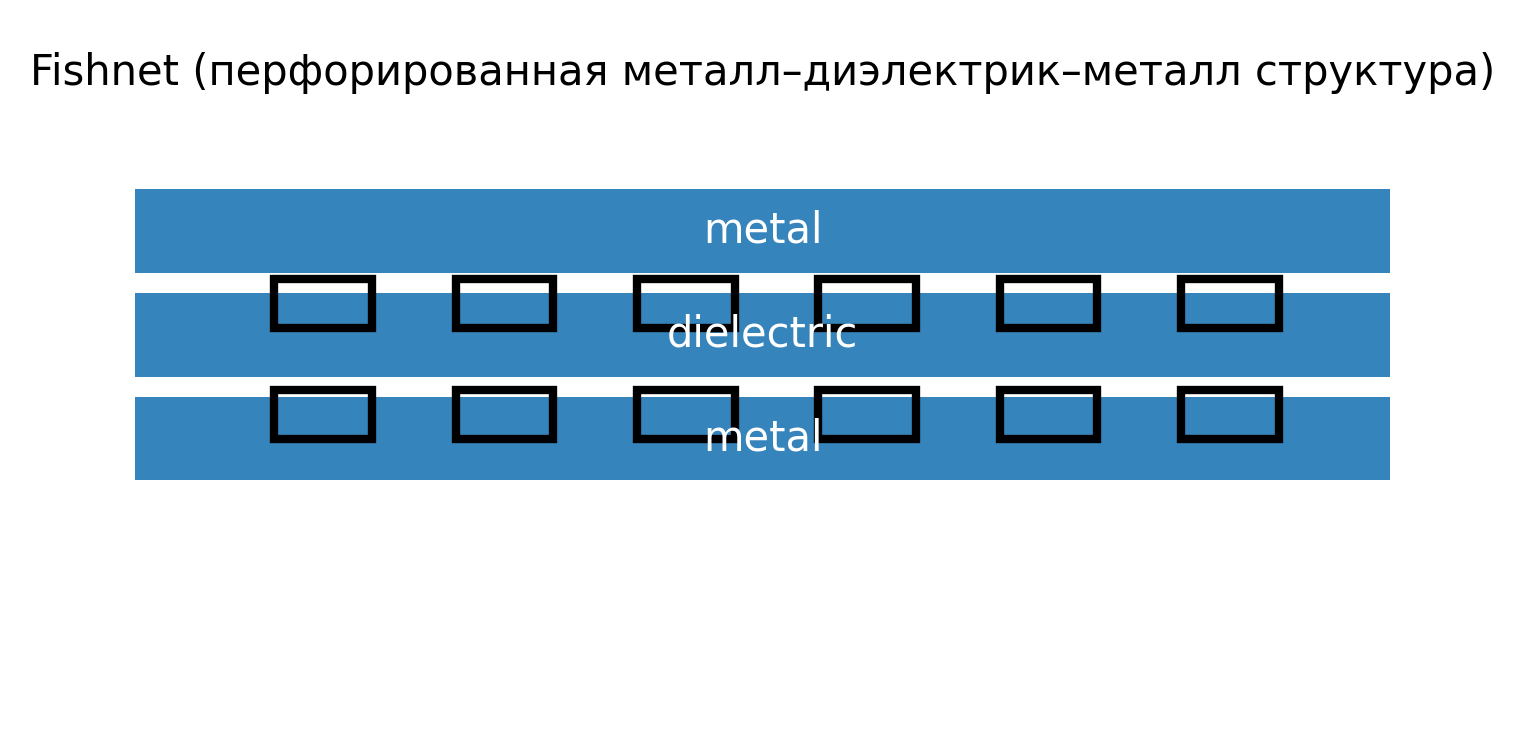
\includegraphics[width=0.70\textwidth]{pictures/fishnet_schematic.png}
        \caption{Схема оптического метаматериала типа \textit{fishnet} (металл--диэлектрик--металл с периодическими отверстиями).\footnote{\url{https://doi.org/10.1038/nphoton.2006.49}}}
        \label{fig:fishnet}
    \end{center}
\end{figure}
\FloatBarrier

\section{Применение метаматериалов}

Основная особенность — возможность создать отрицательную диэлектрическую проницаемость $\varepsilon < 0$ и магнитную проницаемость $\mu < 0$. В результате показатель преломления $n = \sqrt{\varepsilon \mu}$ становится отрицательным. Это ведёт к:
\begin{itemize}
    \item обратному ходу лучей (реверсия закона Снеллиуса),
    \item обратному эффекту Доплера,
    \item левостороннему поведению электромагнитных волн.
\end{itemize}

Такие материалы называют левосторонними (Left-Handed Materials, LHM).


\subsection{Метаповерхности и металинзы (2D-метаматериалы)}
\textbf{Метаповерхность} — это «плоский» метаматериал толщиной $\ll \lambda$, в котором массив нанорезонаторов задаёт локальный фазовый сдвиг и преобразование поляризации. Это позволяет реализовать \textbf{металинзы} (плоские линзы), дефлекторы луча и голограммы в ультратонкой геометрии.\footnote{\url{https://doi.org/10.1038/nmat3839}}
Примером является видимая металинза на основе диэлектрических наностолбиков (TiO$_2$), обеспечивающая дифракционно-ограниченную фокусировку.\footnote{\url{https://doi.org/10.1126/science.aaf6644}}
\begin{figure}[h]
    \begin{center}
        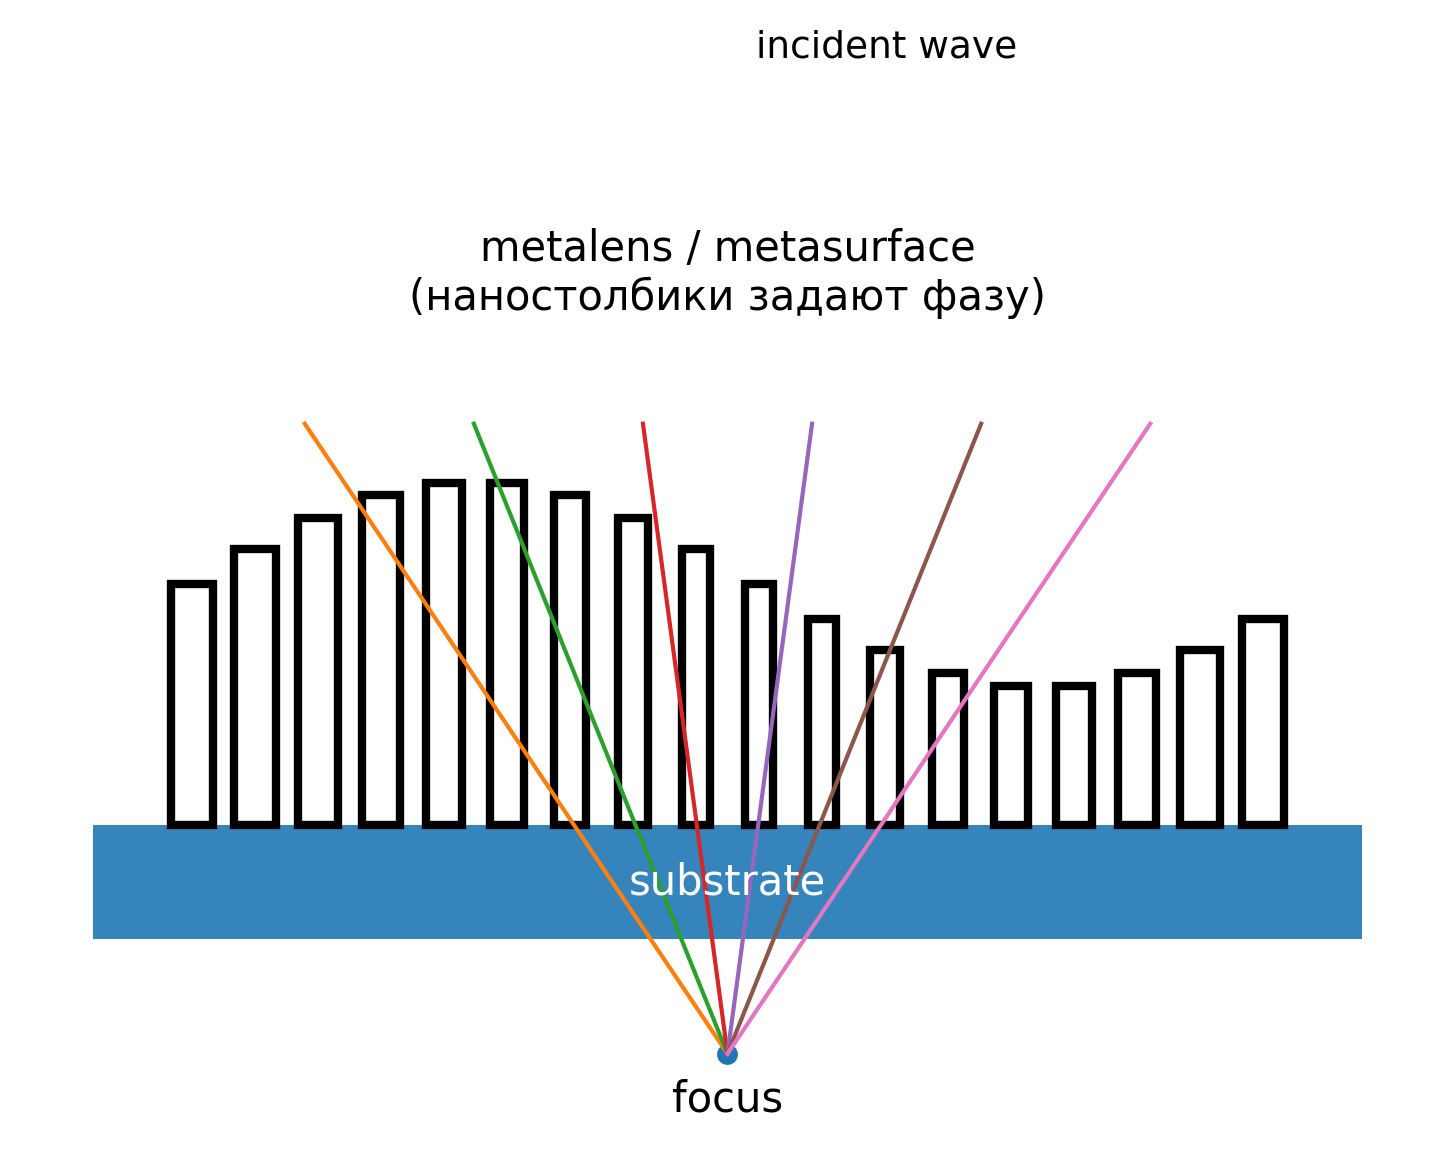
\includegraphics[width=0.80\textwidth]{pictures/metalens_schematic.png}
        \caption{Схема металинзы: параметры элементов метаповерхности (геометрия наностолбиков) задают требуемое распределение фазы и формируют фокус.\footnote{\url{https://doi.org/10.1126/science.aaf6644}}}
        \label{fig:metalens}
    \end{center}
\end{figure}
\FloatBarrier

\subsection{Метаматериальные поглотители (MMA)}

Метаматериальные поглотители — это устройства, способные почти полностью поглощать падающее электромагнитное излучение. Стандартная структура включает:
\begin{enumerate}
    \item верхний слой — металлический рисунок (например, split-ring resonators),
    \item средний — диэлектрик,
    \item нижний — сплошной металлический слой (отражатель).
\end{enumerate}

\begin{figure}[h]
    \begin{center}
        \includegraphics[width = 0.5\textwidth]{pictures/split-ring-resonator.png}
        \caption{Split ring резонатор}
    \label{ust}
    \end{center}
\end{figure}

Поглощение достигается за счёт:
\begin{itemize}
    \item электрических и магнитных резонансов,
    \item согласования импеданса со свободным пространством,
    \item управления плазменной частотой металлов.
\end{itemize}

Применения MMA в оптике:

\begin{itemize}
    \item \textbf{Сенсоры:} MMA чувствительны к изменениям показателя преломления среды.
    \item \textbf{Фотодетекторы и солнечные элементы:} высокая эффективность поглощения.
    \item \textbf{Стелс-технологии:} поглощение СВЧ- и ИК-излучения.
    \item \textbf{Гиперлинзы и суперлинзы:} разрешение ниже дифракционного предела.
\end{itemize}

\section*{Гиперлинзы и сверхразрешение}
\textbf{Гиперлинза} — это тип метаматериального устройства, позволяющего получать изображения с пространственным разрешением, превышающим дифракционный предел. Это достигается за счёт использования \textbf{анизотропных} метаматериалов, у которых компоненты тензора диэлектрической проницаемости имеют \textit{разные знаки}, например:
\begin{equation}
\varepsilon = \begin{pmatrix} \varepsilon_r & 0 & 0 \\ 0 & \varepsilon_\theta & 0 \\ 0 & 0 & \varepsilon_z \end{pmatrix}, \quad \text{где} \quad \varepsilon_r < 0, \ \varepsilon_\theta > 0.
\end{equation}

\begin{figure}[h]
    \begin{center}
        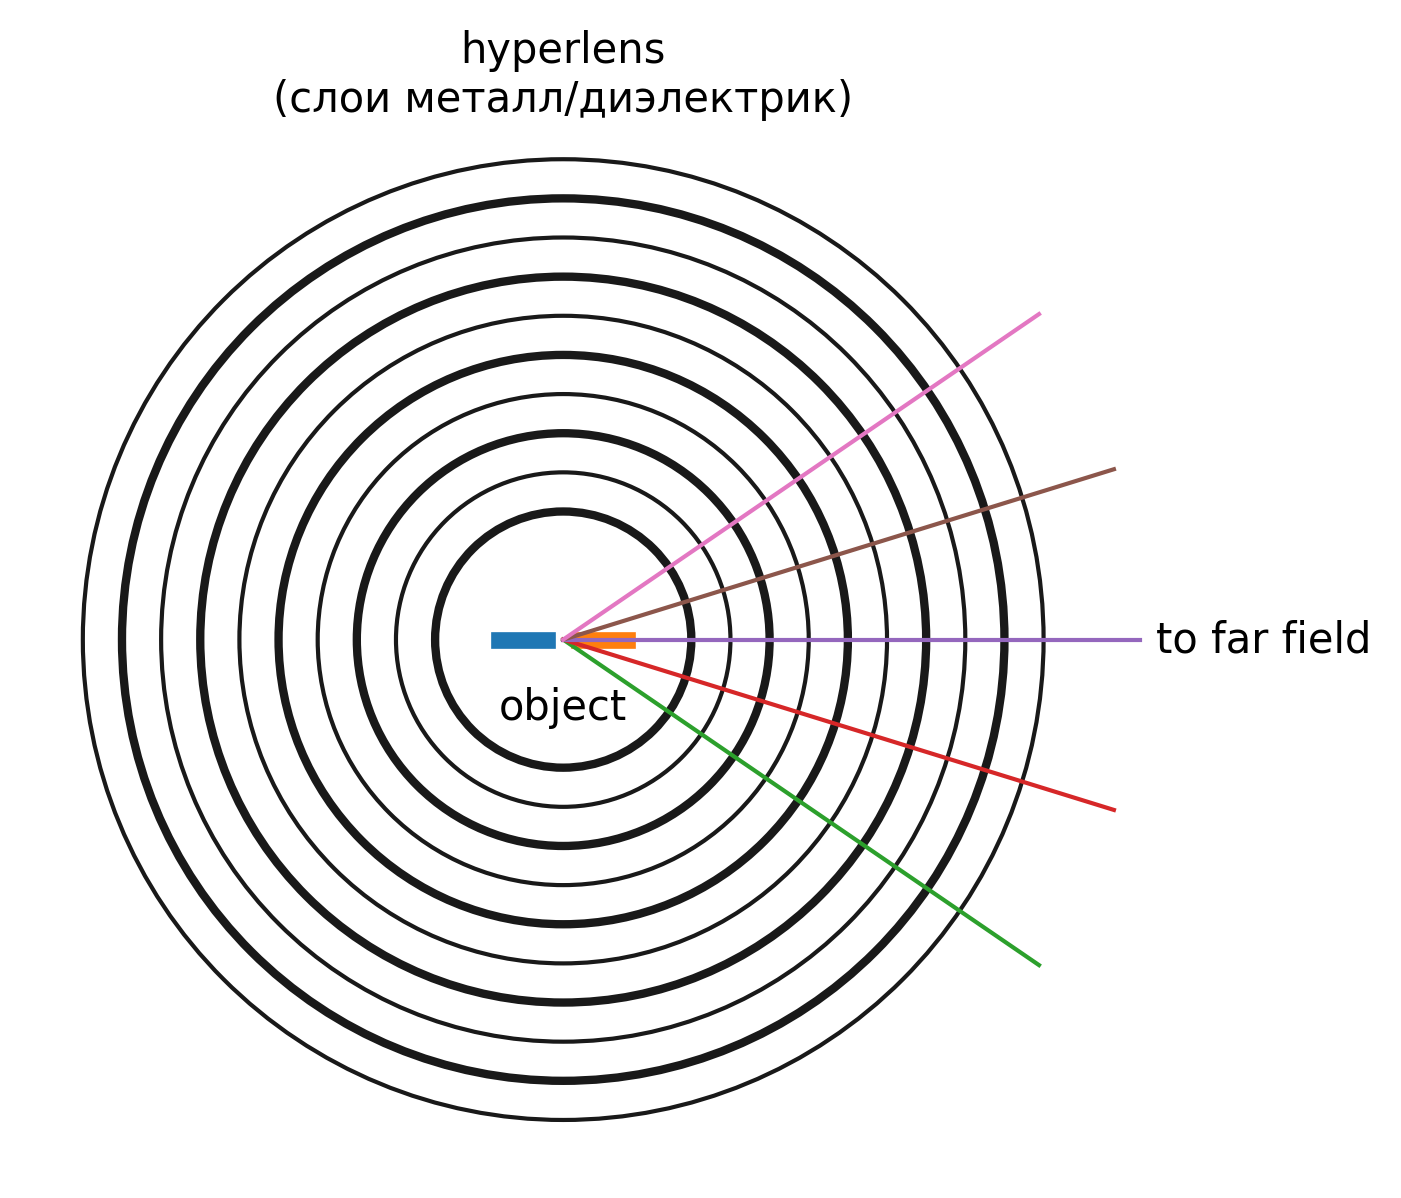
\includegraphics[width=0.55\textwidth]{pictures/hyperlens_schematic.png}
        \caption{Схема гиперлинзы: многослойная цилиндрическая структура металл/диэлектрик переносит субволновые компоненты поля наружу (сверхразрешение).\footnote{\url{https://doi.org/10.1126/science.1137368}}}
        \label{fig:hyperlens}
    \end{center}
\end{figure}
\FloatBarrier

Такая среда называется \textbf{гиперболическим метаматериалом}.

\subsection*{Физика сверхразрешения}
В обычных линзах высокочастотные компоненты изображения (evanescent waves) экспоненциально затухают. Гиперлинза преобразует эти компоненты в \textit{пропагирующие} волны благодаря гиперболической дисперсии:
\begin{equation}
    \frac{k_r^2}{\varepsilon_\theta} + \frac{k_\theta^2}{\varepsilon_r} = \left(\frac{\omega}{c}\right)^2.
\end{equation}
Это гипербола в пространстве волн, в отличие от эллиптической формы в обычных изотропных средах. В результате, высокочастотные волны, несущие субволновую информацию, могут выходить за пределы линзы.

\subsection*{Реализация и применение}
Гиперлинзы реализуются в виде цилиндрических или сферических слоистых структур, где чередуются металлические и диэлектрические слои толщиной $\ll \lambda$. Это обеспечивает эффективную анизотропию.

\begin{itemize}
    \item \textbf{Прямое применение:} визуализация объектов с размером $< \lambda/2$ в реальном времени.
    \item \textbf{Материалы:} серебро/диэлектрик, золото/титан-оксид, графеновые решётки.
    \item \textbf{Области:} биофотоника, нанолитография, флуоресцентная микроскопия.
\end{itemize}

\subsection*{Сравнение с плоской линзой Веселагo}
\begin{itemize}
    \item Веселагo-линза требует $\varepsilon = -1, \mu = -1$ для идеального фокуса.
    \item Гиперлинза работает без необходимости в $\mu < 0$, только на анизотропной $\varepsilon$.
    \item Гиперлинзы проще реализуются на оптических частотах.
\end{itemize}

\section*{Перспективы}

Современные исследования направлены на разработку:
\begin{itemize}
    \item активных и настраиваемых метаматериалов,
    \item голографических метаповерхностей,
    \item компактных устройств для фотоники и ИК-диапазона.
\end{itemize}

Развитие технологий нанофабрикации, включая 3D-печать и литографию, открывает путь к реальному применению в телекоммуникациях, медицинской визуализации и квантовой оптике.

\section*{Заключение}

Метаматериалы представляют собой революционную платформу для управления светом. Особенно интересны метаматериальные поглотители, обладающие высокой эффективностью и компактностью. Эти разработки уже находят применение в реальных устройствах и имеют огромный потенциал в оптике будущего.

На основе уравнений Максвелла в среде с произвольными $\varepsilon$ и $\mu$ получается волновое уравнение $\nabla^2\mathbf{E}-\varepsilon\mu \ \partial^2\mathbf{E}/\partial t^2=0$. Переход к гармоническому виду даёт уравнение Гельмгольца $\nabla^2\mathbf{E}+k^2\mathbf{E}=0$ с $k^2=\omega^2\varepsilon\mu$. Для плоских волн вводится комплексный волновой вектор $k=n\omega/c$ и связанный с ним показатель $n=\pm\sqrt{\varepsilon\mu}$. Фазовая скорость $v_{\text{ф}}=\omega/k=c/n$, групповая $u=d\omega/dk$. Характерный импеданс $Z=\sqrt{\mu/\varepsilon}$ определяет отражение: при равенстве импедансов $Z$ сред отражение отсутствует.

Если $\varepsilon$ и $\mu$ одновременно отрицательны, то $n<0$ и фазовая скорость становится направленной против распространения энергии. В такой левой среде фаза движется противоположно энергии, что приводит к **отрицательному преломлению**: луч света преломляется на ту же сторону от нормали, на которую падает. Вектор Пойнтинга $\mathbf{S}=\mathbf{E}\times\mathbf{H}$ при этом указывает в противоположную сторону относительно $\mathbf{k}$, и группа противофазно переносит энергию в сторону источника. Эти эффекты не учитываются в обычных курсах геометрической оптики и являются характерной чертой метаматериалов с отрицательными $\varepsilon$, $\mu$.



\end{document}
